\documentclass[11pt,a4paper]{article}
\usepackage[margin=2.2cm]{geometry}
\usepackage{graphicx}
\usepackage{hyperref}
\usepackage{enumitem}
\usepackage{booktabs}
\usepackage{xcolor}
\usepackage{float}
\usepackage{setspace}
\singlespacing

\title{\textbf{Assignment 3: Running Oasis 500M --- An Interactive World Model}}
\author{CHEN Long \\ 21321471}
\date{May 2026}

\begin{document}
\maketitle

\section{What I Ran}

I chose \textbf{Oasis 500M} (\texttt{etched-ai/open-oasis} on GitHub), an interactive world model released by Decart and Etched in late 2024. The model generates Minecraft-like gameplay frame by frame, conditioned on keyboard actions---you press W/A/S/D and it generates the next frame accordingly.

\textbf{Hardware:} I rented an Alibaba Cloud ECS GPU instance (ecs.gn7i-c16g1.4xlarge) with a single NVIDIA A10 (24GB VRAM). The actual VRAM usage during inference was around 5.8 GB, so even a 12GB card would have worked fine.

\textbf{Setup:} Mostly smooth, but I ran into three issues. First, the HuggingFace download kept timing out from mainland China, so I had to set \texttt{HF\_ENDPOINT=https://hf-mirror.com} to use a mirror. Second, the repo's \texttt{generate.py} expected the weights in a specific path structure, but my download script put them in a \texttt{./weights/} subfolder---took me about 15 minutes of reading the source code to realize I needed to pass \texttt{--oasis-ckpt} and \texttt{--vae-ckpt} explicitly. Third, \texttt{torchvision 0.26} dropped the \texttt{read\_video}/\texttt{write\_video} API that the repo depends on, so I had to write a compatibility shim using PyAV. That one ate another 20 minutes.

\textbf{Performance:} On the A10, each frame took roughly 0.6--1.5 seconds (faster for early frames, slower as context grows). A 32-frame video (about 1.6 seconds of gameplay at 20fps) took around 29 seconds total. The model weights are 2.3 GB for the DiT and 875 MB for the VAE encoder/decoder.

\begin{figure}[H]
\centering
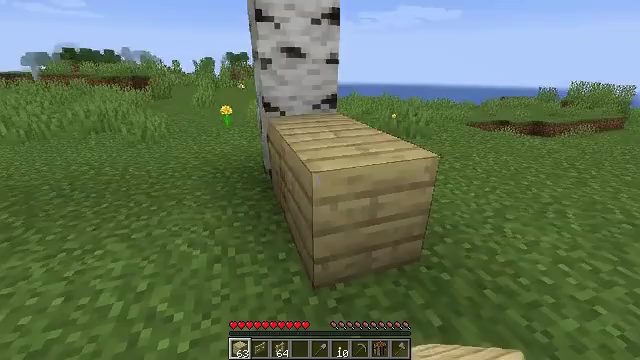
\includegraphics[width=0.48\textwidth]{screenshots/oasis_frame1.png}
\hfill
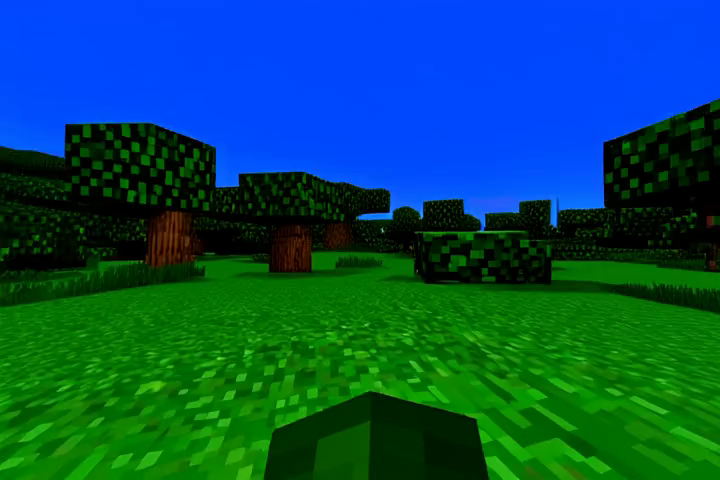
\includegraphics[width=0.48\textwidth]{screenshots/cogvideo_frame1.png}
\caption{Left: Oasis 500M generated frame (action-conditioned world model). Right: CogVideoX-2b generated frame (text-prompted video generation). Both depict Minecraft-style scenes but through fundamentally different generation paradigms.}
\end{figure}

\section{How It Works}

Oasis is built on a \textbf{Spatial-Temporal Diffusion Transformer (DiT)} architecture. Here's the key pipeline:

\begin{enumerate}[nosep]
    \item The current frame is encoded into a latent representation using a ViT-based VAE encoder.
    \item The user's keyboard action (one of several discrete actions like move forward, turn left, jump, etc.) is embedded as a conditioning vector.
    \item The DiT takes the latent of the previous frame(s) plus the action embedding and performs iterative denoising to predict the next frame's latent.
    \item The VAE decoder maps the latent back to pixel space, producing the next visible frame.
\end{enumerate}

What makes this a \textit{world model} rather than just a video generator is the \textbf{action-conditioning loop}. A standard video model (like CogVideoX or Wan2.2) generates an entire clip from a text prompt with no way to intervene mid-generation. Oasis, by contrast, generates one frame at a time in an autoregressive manner, and each frame depends on what action the user took. This creates an interactive simulation---the model has to ``understand'' spatial relationships, physics, and object permanence to respond coherently to player input.

The 500M version uses 2 seconds of context (about 32 frames) as its history window. The full 5B model apparently extends this significantly, but it's not open-sourced.

\section{Observations}

\textbf{What impressed me:}
\begin{itemize}[nosep]
    \item The generated frames genuinely look like Minecraft. Block textures, lighting, sky gradients---all recognizable.
    \item When I used a prompt image of a forest scene and applied ``move forward'' actions, the viewpoint shifted convincingly. Trees got closer, the perspective changed naturally.
    \item The model seems to understand basic depth---objects farther away are smaller and parallax works reasonably.
\end{itemize}

\textbf{What didn't work well:}
\begin{itemize}[nosep]
    \item \textit{Texture flickering:} Block textures shimmer between frames. A grass block might subtly change shade frame-to-frame. It's noticeable when you play the video.
    \item \textit{Object permanence:} If you turn away from something and turn back, it's often different. The model doesn't have a persistent world state---it's just predicting ``what the next frame should look like'' without a real 3D representation.
    \item \textit{Resolution:} 360p output. In 2026 this feels dated. You can see compression artifacts and the overall image is blurry compared to actual Minecraft.
    \item \textit{Long-horizon drift:} After about 20+ frames, the scene starts to lose coherence. Colors shift, geometry gets weird.
\end{itemize}

\begin{figure}[H]
\centering
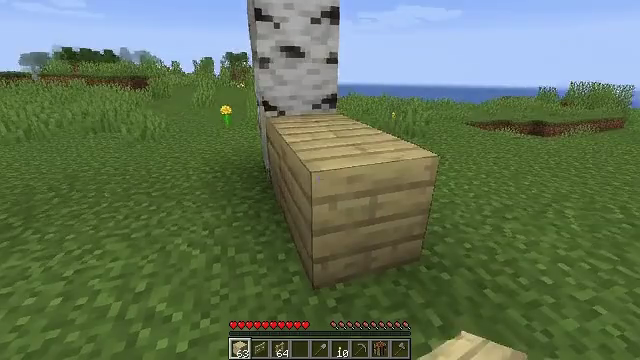
\includegraphics[width=0.45\textwidth]{screenshots/good_frame.png}
\hfill
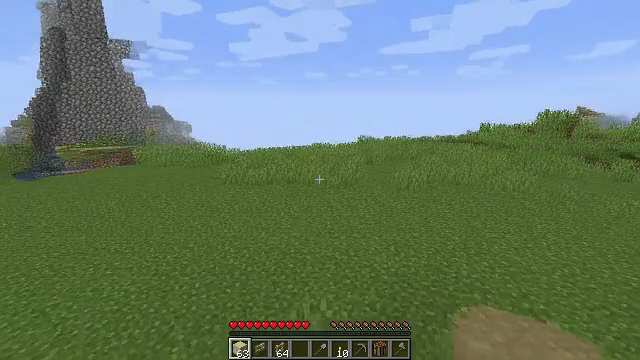
\includegraphics[width=0.45\textwidth]{screenshots/bad_frame.png}
\caption{Left: A well-generated scene at frame 5---clear block textures, coherent structure. Right: After 25 frames of autoregressive generation---note the distorted geometry on the left structure and the overall loss of detail.}
\end{figure}

\section{Reflection}

Back in Assignment 1, I built a tiny ViT from scratch---64-dim embeddings, 2 transformer blocks, 4 attention heads, processing 32$\times$32 images into 10 class logits. It was purely a learning exercise to understand how patch embeddings and self-attention work. Now, seeing Oasis use essentially the same transformer backbone (scaled up massively with diffusion) to generate entire interactive worlds feels like a big conceptual jump. The attention mechanism I visualized in Assignment 1 with those 4$\times$4 patch heatmaps is the same fundamental operation that's now tracking spatial relationships across a 3D game environment.

My understanding has shifted in one key way: I used to think of world models as a fancy label for next-frame prediction. After running Oasis, I realize the hard part isn't generating pretty pixels---CogVideoX can do that too. The hard part is maintaining \textbf{consistency under interaction}. When your model has to respond to arbitrary user actions while keeping the world coherent, that's a fundamentally different problem than generating a fixed video clip.

The biggest gap I see before these models become truly useful: \textbf{persistent spatial memory}. Oasis has no real map or 3D state---it just generates what ``looks right'' based on recent frames. This means it can't handle scenarios like ``go into a house, come back out, and the house should still be there unchanged.'' Solving this probably requires integrating explicit 3D representations (like NeRF or Gaussian Splatting) with the generative model. That hybrid approach seems like the next frontier.

\end{document}
